% The package's structure (README, docs index, report), laid out like the OlmoEarth architecture figure: real imagery
% on the left (Sentinel-2 of scene okavango_80, 1.28 km at 10 m/px, with the frozen-encoder water map, its confidence
% and WorldCover as a second map, from rasters/ as make_rasters.py writes them), the structure on the right (chevrons
% for operations, squares for windows, pink boxes for what the user gets), bold captions under each half.
% Build: pdflatex architecture.tex; export: osascript -l JavaScript pdf2png.js architecture.pdf ../architecture.png 3600
\documentclass[tikz,border=3mm]{standalone}
\usepackage[T1]{fontenc}
\usepackage{helvet}
\renewcommand{\familydefault}{\sfdefault}
\usepackage{amssymb}
\usepackage{graphicx}
\pagecolor{white}
\usetikzlibrary{positioning,arrows.meta,shadows,shapes.geometric,shapes.symbols,calc,fit,backgrounds}
\definecolor{ink}{HTML}{1F2937}\definecolor{muted}{HTML}{6B7280}
\definecolor{s2}{HTML}{E2559B}\definecolor{mapo}{HTML}{F59E0B}\definecolor{pinkout}{HTML}{E94E9B}
\definecolor{teal}{HTML}{0F766E}\definecolor{amber}{HTML}{D97706}\definecolor{violet}{HTML}{6D28D9}
\definecolor{red}{HTML}{DC2626}\definecolor{green}{HTML}{16A34A}\definecolor{sky}{HTML}{BFDBFE}
\hyphenpenalty=10000 \exhyphenpenalty=10000
\tikzset{
  >=Stealth, font=\small,
  flow/.style={->, line width=0.8pt, draw=ink},
  panel/.style={draw=ink!25, dashed, fill=ink!2, line width=0.6pt},
  ptitle/.style={font=\normalsize\bfseries, text=ink, inner sep=1pt},
  caption/.style={font=\large\bfseries, text=ink, inner sep=1pt},
  img/.style={inner sep=0pt, line width=1.3pt, drop shadow={shadow xshift=1.0mm, shadow yshift=-1.0mm, opacity=0.25}},
  thumb/.style={img, draw=mapo, line width=1.4pt},
  tlabel/.style={font=\footnotesize, text=ink, inner sep=1pt},
  op/.style={signal, signal to=east, signal from=west, draw=ink, fill=#1, line width=0.8pt,
             minimum height=9mm, text width=1.55cm, align=center, font=\scriptsize, inner xsep=1pt},
  op/.default=white,
  result/.style={draw=ink, dashed, fill=pinkout, text=white, rounded corners=2pt, line width=0.8pt, minimum height=10mm,
              text width=3.35cm, align=center, font=\footnotesize, drop shadow={shadow xshift=0.6mm, shadow yshift=-0.6mm, opacity=0.2}},
  tok/.style={draw=ink!70, line width=0.5pt, minimum size=3.9mm, inner sep=0pt},
  note/.style={font=\scriptsize, text=muted, align=center, inner sep=1pt},
  part/.style={draw=ink, line width=0.8pt, drop shadow={shadow xshift=0.8mm, shadow yshift=-0.8mm, opacity=0.25}},
  lane/.style={draw=ink!25, dashed, rounded corners=4pt, line width=0.6pt},
  lanetitle/.style={font=\footnotesize\bfseries, text=ink, inner sep=1pt, anchor=north west},
}
\begin{document}
\begin{tikzpicture}

  % ======================================================================= your data and model
  \node[ptitle] at (2.25,8.55) {Satellite observations};
  \begin{scope}[on background layer] \draw[panel] (0.15,2.45) rectangle (4.35,8.15); \end{scope}
  \node[img, draw=s2!55] (bs) at (2.75,5.75) {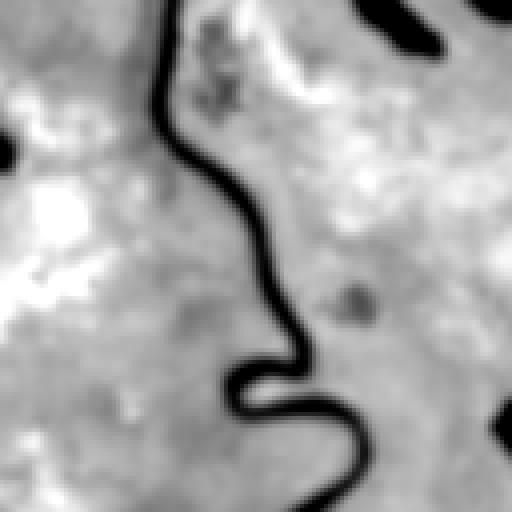
\includegraphics[width=2.55cm]{rasters/scene_b11.png}};
  \node[img, draw=s2!75] (bn) at (2.47,5.47) {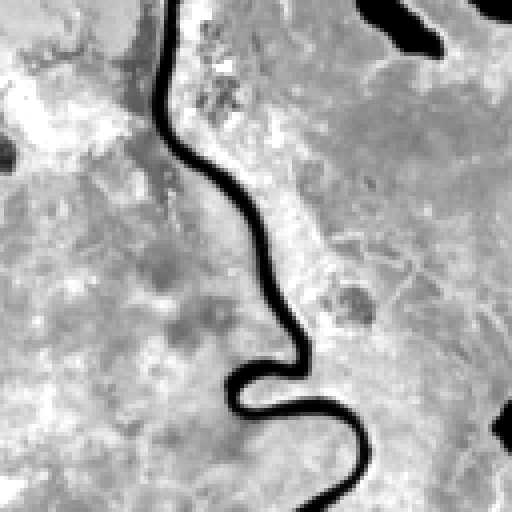
\includegraphics[width=2.55cm]{rasters/scene_b08.png}};
  \node[img, draw=s2] (br) at (2.19,5.19) {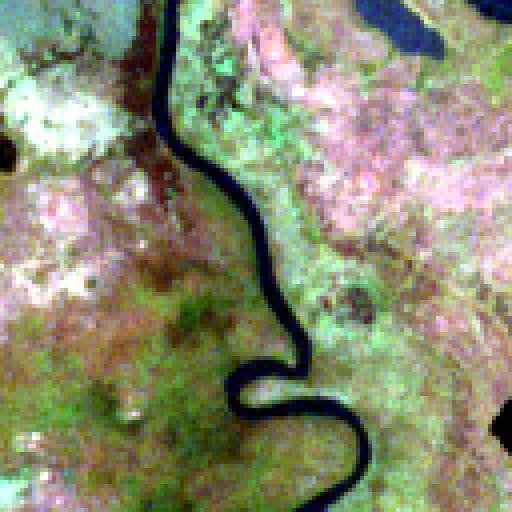
\includegraphics[width=2.55cm]{rasters/scene_rgb.png}};
  \node[font=\scriptsize\bfseries, text=white, anchor=north east, inner sep=2pt] at (br.north east) {10\,m/px};
  \node[font=\normalsize\bfseries, rotate=90, text=ink] at (0.5,5.19) {Sentinel-2};
  \draw[ink!60, |-|, line width=0.5pt] ($(br.south west)+(0,-0.2)$) -- ($(br.south east)+(0,-0.2)$)
        node[midway, below, font=\scriptsize, text=muted] {1.28\,km};
  \node[note, anchor=north] at (2.25,3.15) {RGB $\cdot$ near-infrared $\cdot$\\ short-wave infrared};

  % the model: encoder narrows, decoder widens, names inside
  \draw[flow] (4.42,5.19) -- (4.7,5.19);
  \draw[part, fill=ink!10] (4.78,3.85) -- (4.78,6.55) -- (5.55,5.85) -- (5.55,4.55) -- cycle;
  \draw[part, fill=ink!10] (5.72,4.55) -- (5.72,5.85) -- (6.49,6.55) -- (6.49,3.85) -- cycle;
  \node[font=\footnotesize\bfseries, text=ink, rotate=90] at (5.12,5.2) {Encoder};
  \node[font=\footnotesize\bfseries, text=ink, rotate=90] at (6.15,5.2) {Decoder};
  \node[note] at (5.63,3.35) {any EO model};
  \draw[flow] (6.55,5.19) -- (6.85,5.19);

  % model outputs: real maps in orange frames
  \node[ptitle] at (8.65,8.55) {Model outputs};
  \begin{scope}[on background layer] \draw[panel] (6.95,2.45) rectangle (10.35,8.15); \end{scope}
  \node[tlabel] at (7.85,7.85) {Class map};
  \node[thumb] (pred) at (7.85,6.95) {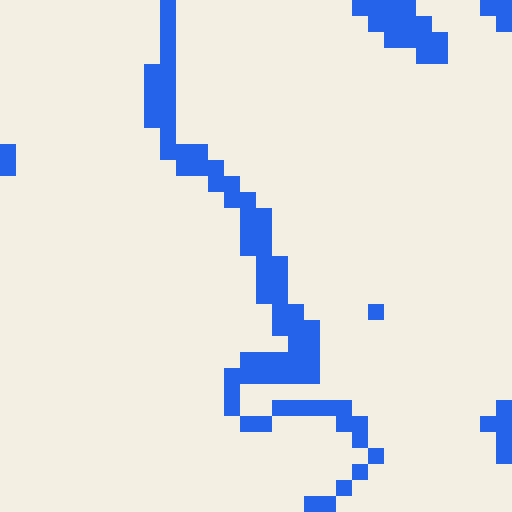
\includegraphics[width=1.4cm]{rasters/scene_pred.png}};
  \node[tlabel] at (9.45,7.85) {Confidence};
  \node[thumb] (conf) at (9.45,6.95) {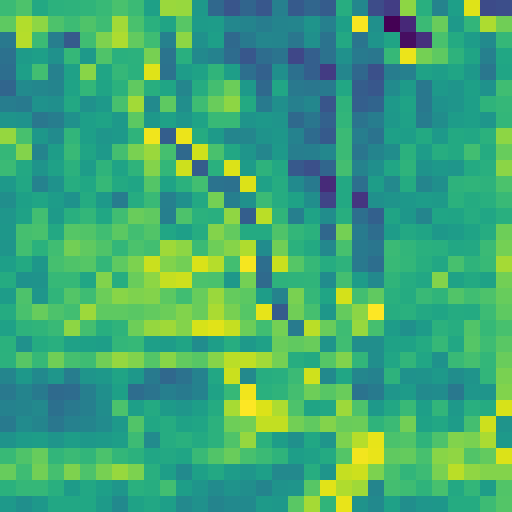
\includegraphics[width=1.4cm]{rasters/scene_conf.png}};
  \node[tlabel] at (7.85,5.6) {Second map};
  \node[thumb] (map2) at (7.85,4.7) {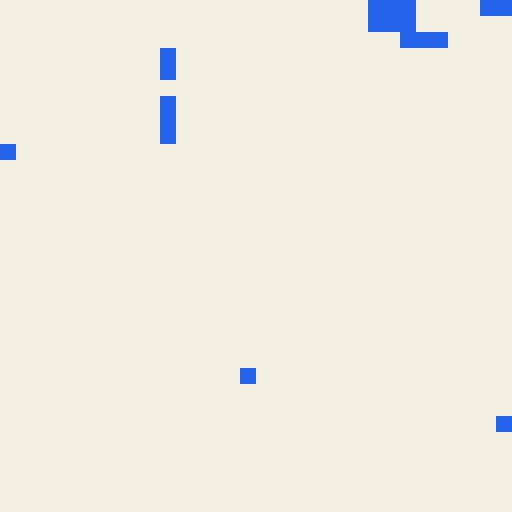
\includegraphics[width=1.4cm]{rasters/scene_label.png}};
  \node[note] at (7.85,3.65) {e.g.\ WorldCover\\ \textit{(optional)}};
  \node[tlabel] at (9.45,5.6) {Condition};
  \node[draw=mapo, dashed, line width=1.2pt, minimum size=1.4cm, inner sep=0pt, fill=white] (cnd) at (9.45,4.7) {};
  \node[note] at (cnd) {e.g.\ cloud\\ flag};
  \node[note] at (9.45,3.65) {per pixel\\ \textit{(optional)}};
  \node[caption] at (5.25,1.85) {Your data and model};

  % ======================================================================= olmoearth-inferenceX
  \draw[flow] (10.42,5.19) -- (10.7,5.19);
  \node[op=sky] (pool) at (11.85,5.19) {Pool to\\ windows};
  \begin{scope}[shift={(11.51,3.55)}]
    \foreach \i in {0,...,3} \foreach \j in {0,...,3} \draw[ink!50, fill=sky!60, line width=0.3pt] (0.17*\i,0.17*\j) rectangle ++(0.17,0.17);
    \draw[ink, line width=0.8pt] (0,0) rectangle (0.68,0.68);
  \end{scope}
  \node[note, anchor=north] at (11.85,3.5) {4\,$\times$\,4 pixels};
  \foreach \s [count=\i] in {90,35,80,20,95,60} {\node[tok, fill=teal!\s!white] (w\i) at (13.6,{6.3-0.42*\i}) {};}
  \draw[flow] (pool.east) -- ($(w3.west)!0.5!(w4.west)$);
  \node[note, anchor=north] at (13.6,3.55) {class +\\ confidence};
  \draw[line width=0.9pt, draw=ink] ($(w3.east)!0.5!(w4.east)$) -- (14.15,5.19);
  \draw[line width=0.9pt, draw=ink] (14.15,7.9) -- (14.15,2.6);

  % ---- no labels
  \draw[lane] (14.4,6.15) rectangle (26.2,8.95);
  \node[lanetitle] at (14.5,8.9) {Without reference labels};
  \node[op] (rank) at (15.65,7.9) {Rank by\\ confidence};
  \draw[flow] (14.15,7.9) -- (rank.west);
  \foreach \s [count=\i] in {20,32,45,60,74,86,94} {\node[tok, fill=teal!\s!white] (r\i) at ({16.8+0.42*\i},7.9) {};}
  \draw[draw=pinkout, line width=1.3pt] ($(r1.south west)+(-0.05,-0.05)$) rectangle ($(r2.north east)+(0.05,0.05)$);
  \node[note, anchor=south] at ($(r1.north)!0.5!(r2.north)+(0,0.08)$) {lowest confidence first};
  \draw[flow] (rank.east) -- (r1.west);
  \node[result, anchor=west] (o1) at (22.40,7.9) {\textbf{Review set}\\ windows to inspect first};
  \draw[flow] (r7.east) -- (o1.west);
  \node[op] (cmp) at (15.65,6.75) {Compare\\ A and B};
  \draw[flow] (14.15,6.75) -- (cmp.west);
  \foreach \d [count=\i] in {0,1,0,1,1,0,0} {\node[tok, fill=\ifcase\d white\or red!35\fi] (c\i) at ({16.8+0.42*\i},6.75) {};}
  \draw[flow] (cmp.east) -- (c1.west);
  \node[result, anchor=west] (o2) at (22.40,6.75) {\textbf{Disagreement map}\\ rate, location, boundaries};
  \draw[flow] (c7.east) -- (o2.west);

  % ---- with a few labels
  \draw[lane] (14.4,2.0) rectangle (26.2,5.9);
  \node[lanetitle] at (14.5,5.85) {With a labelled sample};
  \node[op] (samp) at (15.65,4.85) {Random\\ sample};
  \draw[flow] (14.15,4.85) -- (samp.west);
  \foreach \m [count=\i] in {1,1,0,1,2,1} {
     \node[tok, fill=white, draw=violet, line width=0.8pt] (q\i) at ({16.8+0.42*\i},4.85) {};
     \ifcase\m \node[text=red, font=\scriptsize\bfseries, inner sep=0pt] at (q\i) {$\times$}; \or
       \node[text=green, font=\scriptsize\bfseries, inner sep=0pt] at (q\i) {$\checkmark$}; \or
       \node[font=\scriptsize\bfseries, inner sep=0pt] at (q\i) {?}; \fi}
  \node[note, anchor=south, text=violet] at ($(q3.north)!0.5!(q4.north)+(0,0.08)$) {reference labels: 1, 0 or ?};
  \draw[flow] (samp.east) -- (q1.west);
  \node[op] (est) at (20.95,4.85) {Exact\\ interval};
  \node[op] (cert) at (20.95,3.75) {Exact zone\\ tests};
  \draw[flow] (q6.east) -- (est.west);
  \draw[flow] ($(q6.east)+(0.18,0)$) |- (cert.west);
  \node[result, anchor=west] (o3) at (22.40,4.85) {\textbf{Error rate}\\ with exact 95\% interval};
  \node[result, anchor=west] (o4) at (22.40,3.75) {\textbf{Certified zone}\\ error $\leq\alpha$ (prob.\ $\geq 1-\delta$)};
  \draw[flow] (est.east) -- (o3.west);
  \draw[flow] (cert.east) -- (o4.west);
  \node[op] (dsamp) at (15.65,2.6) {Sample\\ A $\neq$ B};
  \draw[flow] (14.15,2.6) -- (dsamp.west);
  \foreach \m [count=\i] in {1,1,0,1,1} {
     \node[tok, fill=red!15, draw=violet, line width=0.8pt] (p\i) at ({16.8+0.42*\i},2.6) {};
     \node[font=\scriptsize\bfseries, inner sep=0pt] at (p\i) {\ifcase\m B\or A\fi};}
  \node[note, anchor=south, text=violet] at ($(p3.north)+(0,0.08)$) {correct map: A or B};
  \draw[flow] (dsamp.east) -- (p1.west);
  \node[op] (diff) at (20.95,2.6) {Interval on\\ the difference};
  \draw[flow] (p5.east) -- (diff.west);
  \node[result, anchor=west] (o5) at (22.40,2.6) {\textbf{Accuracy difference}\\ A $-$ B, 95\% interval};
  \draw[flow] (diff.east) -- (o5.west);

  \node[caption] at (20.3,1.45) {olmoearth-inferenceX};
\end{tikzpicture}
\end{document}
